\PassOptionsToPackage{force}{filehook}

\documentclass{beamer}
\setbeamersize{text margin left=5mm,text margin right=5mm}
\usecolortheme{wolverine}
\setbeamertemplate{footline}[frame number]
%\useoutertheme{split}
\useinnertheme{rounded}
\usepackage{pgf,tikz}
\usetikzlibrary{positioning}
\usepackage{amsmath}
\usepackage{amsfonts}
\usepackage{graphicx} 
\usepackage{subcaption}
\usepackage{hyperref}
\usepackage{cancel}
\usepackage{wrapfig}
\usepackage{comment}
\hypersetup{
	colorlinks=true,
	linkcolor=blue,
	filecolor=magenta,      
	urlcolor=cyan,
}
\usepackage{color}
\usepackage{mathpazo}
\usepackage{hyperref}
\usepackage{multimedia}
\usepackage{graphicx}
%\usepackage[demo]{graphicx}
\usepackage{caption}
\usepackage{subcaption}
\usepackage{textcomp}
\usepackage{graphicx} 
\usepackage{booktabs}
\usepackage{cite}
\usepackage{hyperref}
\usepackage{multicol}
\usepackage{multirow,array}
\usepackage{amsmath}
\usepackage{mathrsfs}
\usepackage{amssymb}
\usepackage[utf8]{inputenc}
\usepackage{amsthm}
\usepackage{halloweenmath}
\newtheorem{thm}{Teorema}
\newtheorem{lem}[thm]{Lema}
\newtheorem{axiom}[thm]{Axioma}
\newtheorem{prop}[thm]{Proposici\'on}
\newtheorem{cor}[thm]{Corolario}
\theoremstyle{definition}
\newtheorem{defn}{Definici\'on}
\DeclareGraphicsExtensions{.pdf,.jpeg,.png,.eps}
%\usetheme{CambridgeUS}
\setbeamertemplate{navigation symbols}{}
\usepackage{pgf,tikz}
\usetikzlibrary{positioning}
\usepackage[spanish, activeacute]{babel} %Definir idioma español
\usepackage[utf8]{inputenc} %Codificacion utf-8
\usepackage{multirow}
\def\mydate{\leavevmode\hbox{\twodigits\day/\twodigits\month/\the\year}}
\def\twodigits#1{\ifnum#1<10 0\fi\the#1}
\definecolor{rosee}{rgb}{0.7,0.05,0.25}
\usepackage[final]{pdfpages}

%   Esconder las soluciones
\newif\ifhideproofs
\hideproofstrue %uncomment to hide proofs

\ifhideproofs
\usepackage{environ}
\NewEnviron{hide}{}
\let\solucion\hide
\let\endsolucion\endhide
\fi

\usepackage{enumitem}

\title{Microeconomía}
\subtitle{Teoría de la firma - Tecnología de producción\footnote{Basado en notas de Marcos Lissauer}\\ \mydate}
\author[Tecnología de producción]{Lara Sánchez Peña}
\date{ Universidad Torcuato di Tella}

\begin{document}
	\frame{\titlepage}
	
\begin{frame}{Un poco de humor: el que avisa no traiciona... $\mathwitch$}
    \begin{center}
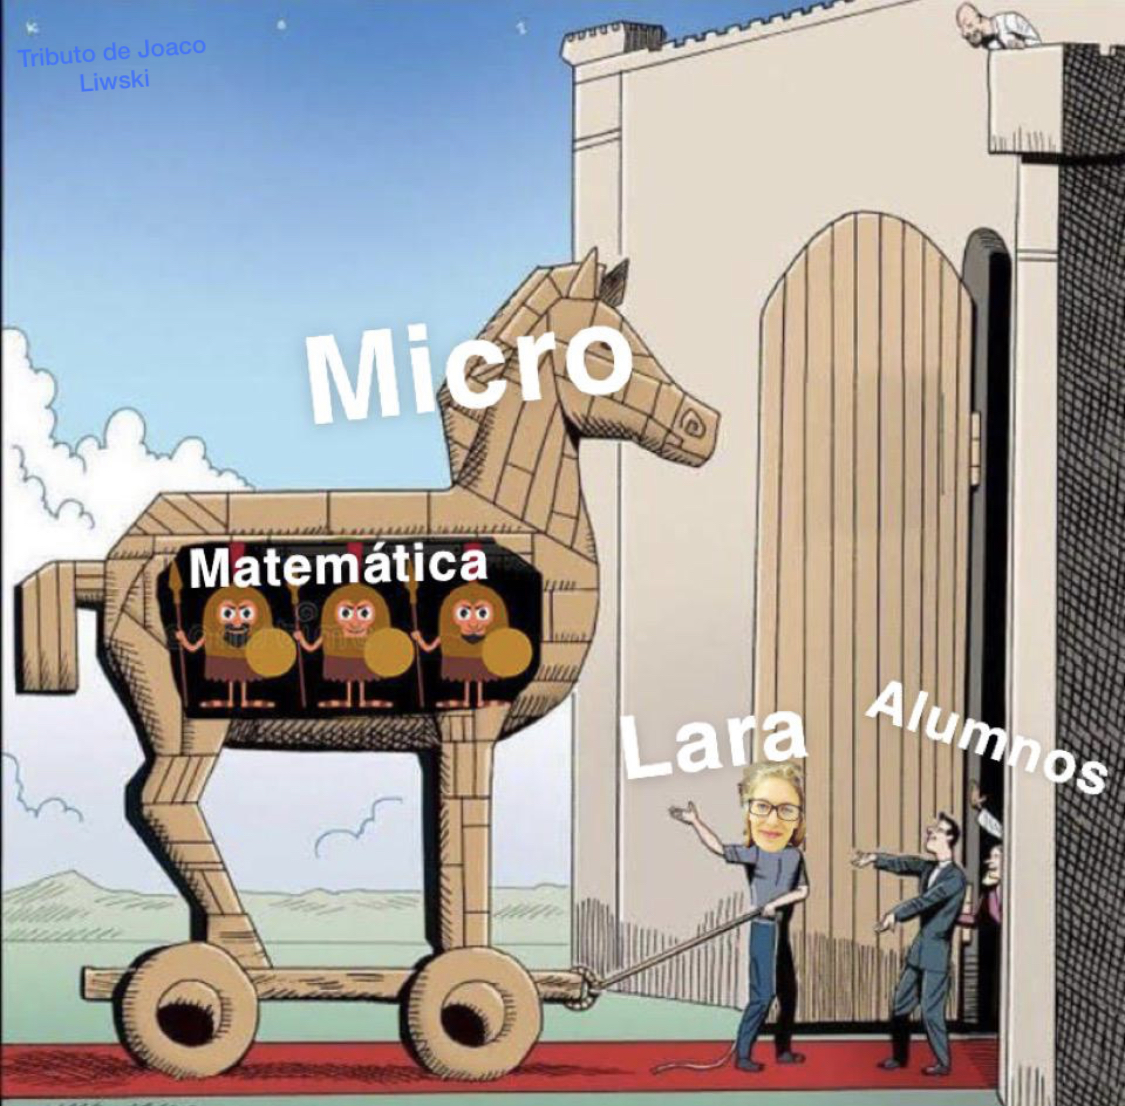
\includegraphics[width=3in]{figures2/meme1.jpg}
\end{center}
\end{frame}	
	\begin{frame}{Objetivos de estas slides 1 de 2}
    \begin{itemize}
        \item ¿Qué es una tecnología de producción que usa insumos $(x_1,x_2)$ y produce un bien final $y$ (también llamado $q$)?
        \item ¿Cómo se llama el conjunto de todas las combinaciones de $(x_1,x_2,y)$ que la tecnología permite producir? \textbf{Conjunto de producción}.%; FPP; planes de producción eficientes, ineficientes, inalcanzables.
        % \item \textbf{Costo de oportunidad sobre la FPP: TMT}
        \item ¿Cómo se llama el conjunto de todas las combinaciones de $(x_1,x_2)$ que permiten producir una cantidad específica $\overline{y}$? \textbf{Isocuanta}.
        \item Ejemplos de tecnología e isocuantas asociadas.
        \item Propiedades del conjunto de producción: \textbf{monotonicidad y convexidad}.
\item Supongamos que tenemos $(x_1,x_2)$ y producimos $f(x_1,x_2)$ y consideramos agregar una unidad más del insumo 1, ¿cuánto es el \textbf{aumento} en la cantidad producida? \textbf{Productividad marginal del insumo} $1$, $PMg(x_1,x_2)$.
        \end{itemize}
        \end{frame}
        	\begin{frame}{Objetivos de estas slides 2 de 2}\small
    \begin{itemize}

        \item Supongamos que queremos producir una cantidad $\overline{y}$ fija sobre una isocuanta, consideramos dejar de utilizar una unidad del insumo $1$. Con tal de seguir produciendo la cantidad $\overline{y}$, ¿\textbf{Cuántas unidades del insumo $2$ adicionales} tiene que comprar la firma? $TMST(x_1,x_2)$.
         \item Si se multiplican todos los insumos por la misma escala. Por ejemplo, inicialmente se tiene $(x_1,x_2)$ y al aumentar la escala por $t>1$ se tiene de cada insumo $(tx_1,tx_2)$. ¿Cómo se comparan $f(tx_1,tx_2)$ y $t\cdot f(x_1,x_2)$ ? La respuesta depende de los \textbf{rendimientos a escala (RS).}
         \item Tecnologías donde es fácil determinar los rendimientos a escala: En las \textbf{tecnologías homogéneas de grado} $k$ (\textbf{HOD} $k$) vale que $f(tx_1,tx_2)=t^kf(x_1,x_2)$. 
         \item Una \textbf{tecnología} $h$ es \textbf{homotéticas} si $h(x_1,x_2)=g(f(x_1,x_2))$ con $g$ una función creciente y $f(x_1,x_2)$ una función \textbf{HOD} $k$.
        \item Relación entre los RS y el conjunto de producción.
        \item Material de repaso: Ver slides de Eco 1 5.1.
    \end{itemize}
\end{frame}

%\begin{frame}{Introducci\'on}
%\begin{itemize}
%\item En esta secci\'on iniciamos el estudio del comportamiento de la empresa. Lo primero que debemos hacer es \textbf{analizar las limitaciones con que se encuentra la firma cuando toma sus decisiones}. Estos límites vienen impuestos por sus clientes, por los competidores y por la ``naturaleza''.
%\item En particular, en esta secci\'on analizaremos el efecto de la naturaleza en la toma de decisiones de la firma. La naturaleza impone restricciones, ya que sólo existen \textbf{ciertas formas viables de producir bienes a partir de factores}, es decir, sólo son posibles determinados tipos de \textbf{elecciones tecnológicas}. Analizaremos c\'omo describimos las \textbf{restricciones tecnol\'ogicas}.
%\end{itemize}
%\end{frame}

\begin{frame}{Tecnología de producción}
	\begin{itemize}

		\item Definimos \textbf{una tecnología de producción} al proceso que permite \textbf{transformar insumos}\footnote{También llamados factores de producción. Notación: $\textbf{x}=(x_{1},x_{2},...x_{n})$.} $(x_{1},x_{2},...x_{n})$ \textbf{en un bien final} $y$.\footnote{También llamado $q$.}


   \item La tecnología de producción se describe por medio de la \textbf{función de producción} $f(\textbf{x})$. Indica la máxima cantidad de producto que la firma puede producir con $\textbf{x}$ insumos.
   
		\item La tecnolog\'{\i}a \textbf{limita las posibilidades de producci\'{o}n de la firma} ya que establece qu\'{e} cantidad de producto final es posible obtener dada la cantidad de insumos elegida.

		\item Por ejemplo, para producir una computadora $(y)$ necesitamos plástico $(x_{1})$, metal $(x_{2})$ e ingenieros $(x_{3})$. Por lo tanto, el vector de insumos es $\textbf{x}=(x_1,x_2,x_3)$. La cantidad máxima de computadoras que se puede producir con esa cantidad de insumos es $f(x_1,x_2,x_3)$.
  
		
	\end{itemize}
\end{frame}


\begin{frame}{Función de producción}
	\begin{itemize}
		\item Definimos un \textbf{plan de producción} como una combinación de insumos y productos $(\textbf{x},y)$.
		\item Un plan de producción $(\textbf{x},y)$ es \textit{tecnológicamente factible} si $y \leq f(\textbf{x})$. Es decir, con los insumos $\textbf{x}$ se pued producir como máximo una cantidad mayor o igual a $y$.
  
  %si es posible producir $y$ a partir de $\textbf{x}$. Es decir, si dada cierta cantidad de insumos ``n\'{u}mero 1'', ``n\'{u}mero 2'', etc, es posible producir la cantidad de bien final $y$.
		\item Al \textbf{conjunto de planes tecnológicamente factibles} lo llamamos \textbf{conjunto de producción} y lo denotamos $Y$.
		
	\end{itemize}
\end{frame}

\begin{frame}{Conjunto de producción}
	\begin{itemize}
		\item Más formalmente, el conjunto de producción se define como
		$$Y=\lbrace (\textbf{x},y) \in \mathbb{R}^{n+1}: y \leq f(\textbf{x}) \rbrace$$
		\item Si $n=1$ (si la firma usa un solo insumo) podemos graficar fácilmente el conjunto de producción en dos dimensiones, en $\mathbb{R}^2$.
		\\
\begin{center}
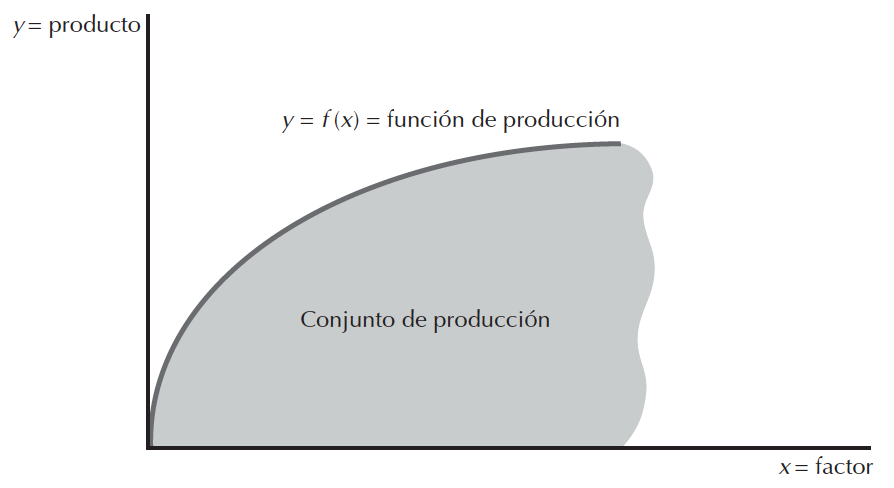
\includegraphics[width=3.8in]{figures2/prodset.png}
\end{center}
	\end{itemize}
\end{frame}

\begin{frame}{Eficiencia en la producción}

	Un plan de producción $(x_{1},...,x_{n},y) \in Y$ (es decir, factible) es (también) \textbf{eficiente} si no existe otro plan $(x'_{1},...,x'_{n},y') \in Y$ tal que $\forall i, x'_{i}\leq x_{i}$ y además $y'\geq y$. O sea, una combinación de insumos y productos es eficiente si no es posible:
 \begin{enumerate}
     \item con la misma cantidad de insumos producir más del bien final,
     \item ni con una menor cantidad de insumos producir la misma cantidad del bien final.
	\begin{itemize}
%	\item Es decir, que un plan de producción es eficiente si no existe otra manera de producir la misma cantidad con menos insumos, o bien, producir más con los mismos insumos.
	\item Concluimos que un plan que cumpla $y < f(\textbf{x})$ no puede ser eficiente. En otras palabras, si un plan es eficiente, entonces debe cumplirse que $y=f(\textbf{x})$.
	\item Sin embargo \textbf{los planes de producción sobre la frontera} del conjunto $Y$ \textbf{pueden o no ser
eficientes}. En las próximas slides veremos de qué depende que sean eficientes o no.

\end{itemize}
\end{enumerate}
\end{frame}

\begin{frame}{Isocuantas}
\textbf{¿Qué es una isocuanta?}
Es el conjunto de todas las combinaciones de $(x_1,x_2)$ que permiten producir una cantidad específica $\overline{y}$ usando una tecnología $f(x_1,x_2)=\overline{y}$.
	\begin{itemize}
		%\item Si tenemos 2 insumos de producci\'on $\textbf{x}=(x_{1},x_{2})$, es de gran utilidad graficar todas las combinaciones de insumos que nos dan la misma cantidad de producto. 
		\item La \textit{isocuanta} para la cantidad $\overline{y}$, son combinaciones de insumos $(x_1,x_2)$ que, a través de la tecnología $f$, permiten producir la \textbf{misma }(iso) \textbf{cantidad} (cuanta) de producto $\overline{y}$.
		\item Matemáticamente,  las isocuantas $\overline{y}=f(x_1,x_2)$ representan las curvas de nivel $\overline{y}$ de la función $f$.
		\item Ejercicios: encuentre las isocuantas si $\overline{y}=8$ para las siguientes tecnologías:
		\begin{enumerate}
		    \item $f(x_1,x_2)=\sqrt{x_1x_2}$
		    \item $f(x_1,x_2)=x_1+2x_2$
		\end{enumerate}
	\end{itemize}
\end{frame}

\begin{frame}{Isocuantas: Tecnología Leontief}
\begin{itemize}
\item La tecnología Leontief es la tecnología en donde los insumos $1$ y $2$ deben usarse en proporciones fijas y los insumos no son sustituibles entre sí. 
\item Imaginemos que en el bar de Mingo el tostado de jamón y queso se hace, \textbf{sin excepción}, con una feta de queso (Q) y una feta de jamón (J). (Un tostado de J\&Q necesariamente tiene que tener ambos ingredientes).
\item ¿Cuántos tostados se producen si a) tenemos una feta de queso y cinco de jamón? b) tenemos cinco fetas de queso y una de jamón?
	\item En ambos casos, seguimos produciendo un tostado.

\item Por lo tanto la función de tecnología es para este caso $f(J,Q)=\min\{J,Q\}$.

\item Si la función de producción de tostados en Havanna es $f(J,Q)=\min\left\{J,\frac{Q}{2}\right\}$. ¿Cuántas fetas de cada ingrediente usa para producir un tostado?


%	\item Imaginemos que queremos realizar agujeros en la tierra y descubrimos que para ello necesitamos una pala y una persona para producir un agujero.
%	\item ¿Qué sucede si le damos a la persona 50 palas? ¿Qué sucede si contratamos 50 personas pero s\'olo una pala?
%	\item En ambos casos, seguimos produciendo 1 agujero. 
%	\item Podemos definir la forma en la que transformamos palas y personas en agujeros con la función de producción $f(L,P)=\min\lbrace L,P\rbrace$.
\end{itemize}
\end{frame}

\begin{frame}{Isocuantas: Tecnología Leontief}
\begin{itemize}
\item La tecnología Leontief se describe con las funciones:\footnote{Esta tecnología se puede generalizar agregando un exponente: $f(x_{1},x_{2})=\left(\min\lbrace ax_{1},bx_{2}\rbrace\right)^{\alpha}; \ a,b>0$.}
$$f(x_{1},x_{2})=\min\lbrace ax_{1},bx_{2}\rbrace; \ a,b>0$$
\end{itemize}	
\begin{center}
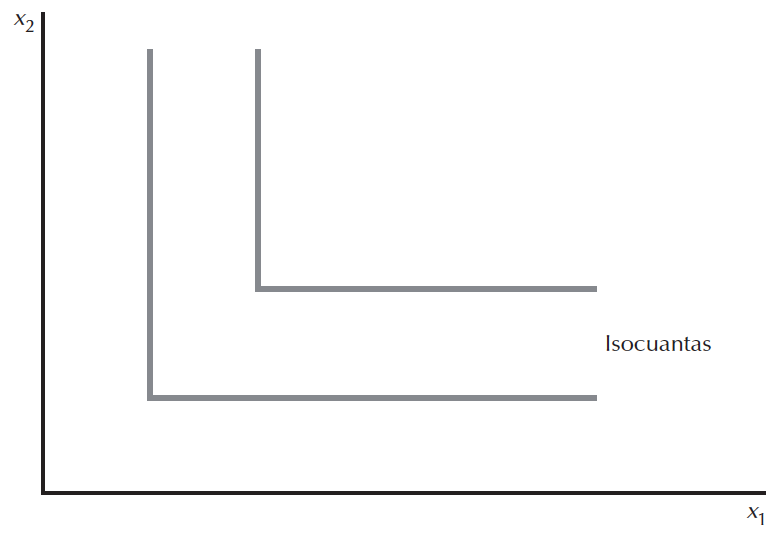
\includegraphics[width=2in]{figures2/leontief.png}
\end{center}
\textbf{Pregunta:} Si se quiere producir $y=a\cdot b$, ¿cuánto se utiliza de cada insumo? 
\end{frame}



\begin{frame}{Isocuantas: Tecnología Leontief}

\begin{figure}
\centering
\begin{subfigure}{.5\textwidth}
  \centering
  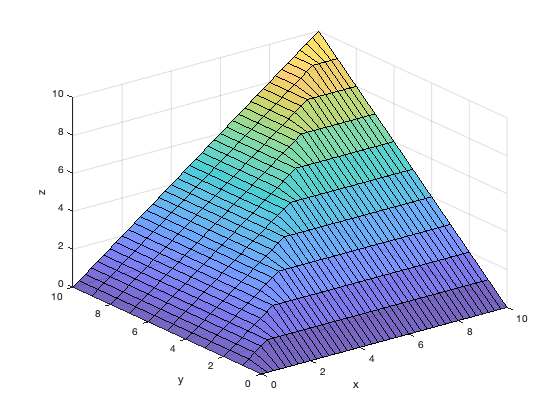
\includegraphics[width=1\linewidth]{figures2/complements3d.png}
  \caption{Función de producción Leontief}
  \label{fig:sub1L}
\end{subfigure}%
\begin{subfigure}{.5\textwidth}
  \centering
  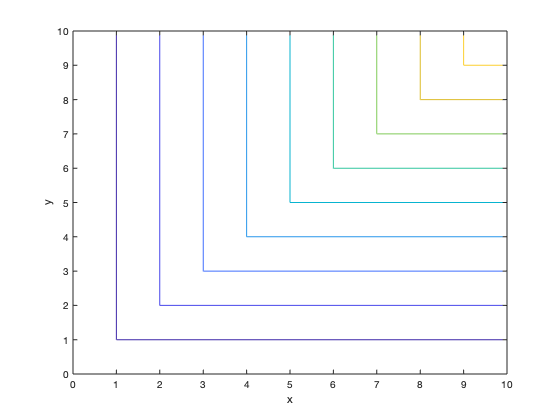
\includegraphics[width=1\linewidth]{figures2/complementslevel.png}
  \caption{Isocuantas Leontief}
  \label{fig:sub2L}
\end{subfigure}
\caption{Tecnología Leontief si $a=1$ y $b=1$.}
\label{fig:testL}
\end{figure}


\end{frame}
\begin{frame}{Tecnolog\'ia Sustitutos Perfectos}
	\begin{itemize}
 \item La tecnología de \textbf{sustitutos perfectos} es la tecnología en donde los insumos $1$ y $2$ son sustituibles (perfectamente) en proporciones fijas.
 \item En el bar de Mingo se usan dos marcas de granos de café, los de Cabrales y los de Illy. $C$ mide la cantidad de granos de Cabrales para producir una taza y $L$ mide la cantidad de granos de Illy para producir una taza. 
 \item Supongamos que para hacer una taza de café se usan $10$ granos de Cabrales y $15$ granos de Illy.
 \item ¿Cuántas tazas de café se producen si
 \begin{itemize}
     \item se usan 100 granos de Cabrales?
     \item se usan 150 granos de Illy?
     \item se usan 40 granos de Cabrales y 90 de Illy?
 \end{itemize}
\item En cualquier caso, se producen 10 cafés.
\end{itemize}
\end{frame}
\begin{frame}{Tecnolog\'ia Sustitutos Perfectos}
	\begin{itemize}
\item Por lo tanto la función de tecnología es para este caso $f(C,L)=\frac{C}{10}+\frac{L}{15}$.

\item ¿Qué insumo es relativamente más eficiente?

\item Si la función de producción de café en Havanna es $f(C,L)=\frac{C}{15}+\frac{L}{10}$. ¿Cuántos granos de café usan para producir un café? Responda para cada marca.
	\end{itemize}
	%	\item Ahora supongamos que queremos publicar un informe mensual de conyuntura macroeconómica.
	%	\item Tanto un estudiante de la Lic. de Economía como de la Lic. de Economía Empresarial pueden escribir un informe por mes.
	%	\item ¿Qué sucede si contranto a un economista y a un economista empresarial? ¿Qué sucede si contrato a 2 economistas? ¿Qué sucede si contrato a 2 economistas empresariales?
	%	\item En cualquiera de los casos anteriores voy a obtener 2 informes.
	%	\item La función que describe la producción de informes es $f(x_{1},x_{2})=x_{1}+x_{2}$, donde $x_i$ son la cantidad de licenciados de cada tipo.

\textbf{Considere ahora otro ejemplo:} Imagine que tiene dos tipos de cartuchos: los truchos ($x_1$) y los originales ($x_2$) que permiten producir hojas impresas ($y$). Un cartucho trucho imprime 500 hojas, mientras que un cartucho original permite imprimir 1500 hojas.
	\begin{itemize}
 \item ¿Cuáles son los coeficientes técnicos de la función de producción que es $f(x_1,x_2)=ax_1+bx_2$?
 \item ¿Qué insumo es relativamente más eficiente?
	\end{itemize}

 
\end{frame}

\begin{frame}{Isocuantas: Tecnolog\'ia Sustitutos Perfectos}
	\begin{itemize}
		\item La función anterior pertenece a una familia más general de funciones de sustitutos:\footnote{Esta tecnología se puede generalizar agregando un exponente: $f(x_{1},x_{2})=\left( ax_{1}+bx_{2}\right)^{\alpha}; \ a,b>0$.} $$f(x_{1},x_{2})=ax_{1}+bx_{2}; \ a,b>0$$
	\end{itemize}
\begin{center}
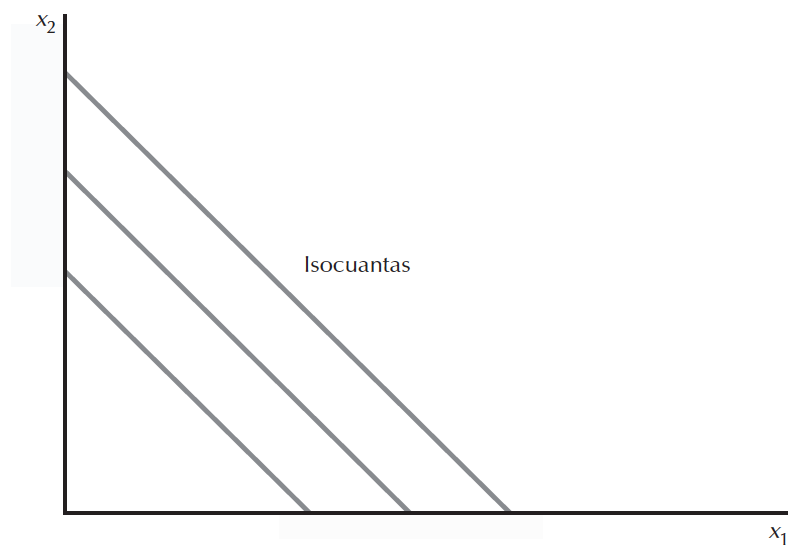
\includegraphics[width=3in]{figures2/sustitutos.png}
\end{center}
\end{frame}

\begin{frame}{Isocuantas: Tecnología Sustitutos Perfectos}
    \begin{figure}
\centering
\begin{subfigure}{.5\textwidth}
  \centering
  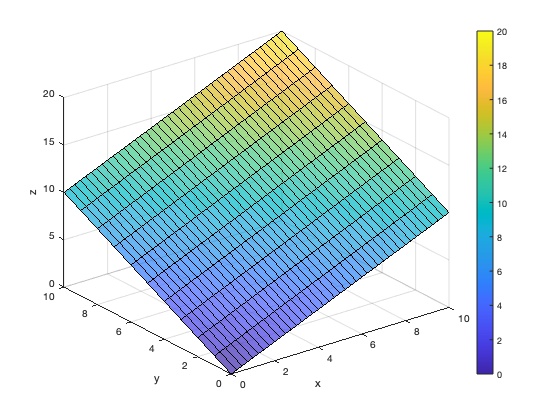
\includegraphics[width=1\linewidth]{figures2/substitutes3d.png}
  \caption{Función de producción de Sustitutos Perfectos}
  \label{fig:sub1S}
\end{subfigure}%
\begin{subfigure}{.5\textwidth}
  \centering
  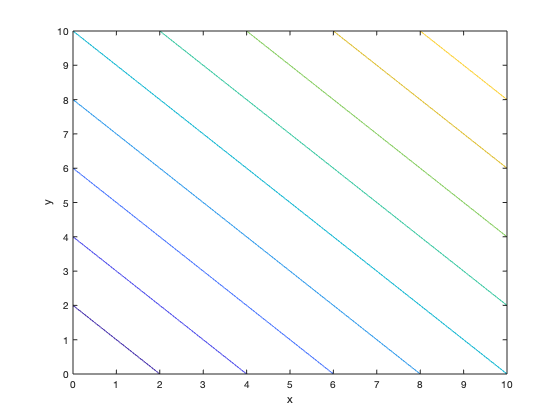
\includegraphics[width=1\linewidth]{figures2/substituteslevel.png}
  \caption{Isocuantas Sustitutos Perfectos}
  \label{fig:sub2S}
\end{subfigure}
\caption{Tecnología Sustitutos Perfectos si $a=1$, $b=1$.}
\label{fig:testS}
\end{figure}
\end{frame}


\begin{frame}{Isocuantas: Tecnolog\'ia Cobb-Douglas}
\begin{itemize}
\item Una tecnología que es una caso intermedio entre la tecnología Leontief y la de sustitutos perfectos es la tecnología Cobb-Douglas. Los dos insumos son complementarios en cierta medida, pero no tanto para ser Leontief.
	%\item Ahora supongamos que los dos insumos requeridos para producir un bien son complementarios en cierta medida, pero no tanto para ser Leontief.
	%\item Adem\'as, la tasa a la que puedo sustituir un bien por otro depende de la cantidad utilizada.
	\item La tecnología Cobb-Douglas se representa con las funciones:
		$$f(x_{1},x_{2})=Ax_{1}^{\alpha}x_{2}^{\beta}; \ \alpha,\beta > 0$$
	\item El parámetro $A$ mide, aproximadamente, la escala de producción, es decir, el volumen de producción
que se obtiene si se utiliza una unidad de cada factor. 

\item Los parámetros $\alpha$ y $\beta$ indican los siguiente: si $\alpha$ es mayor a $\beta$, más de la mitad de los costos totales se deberán a la cantidad comprada de insumo $1$.
\end{itemize}
\end{frame}

%\begin{frame}{Isocuantas: Tecnolog\'ia Cobb-Douglas}
%\begin{center}
%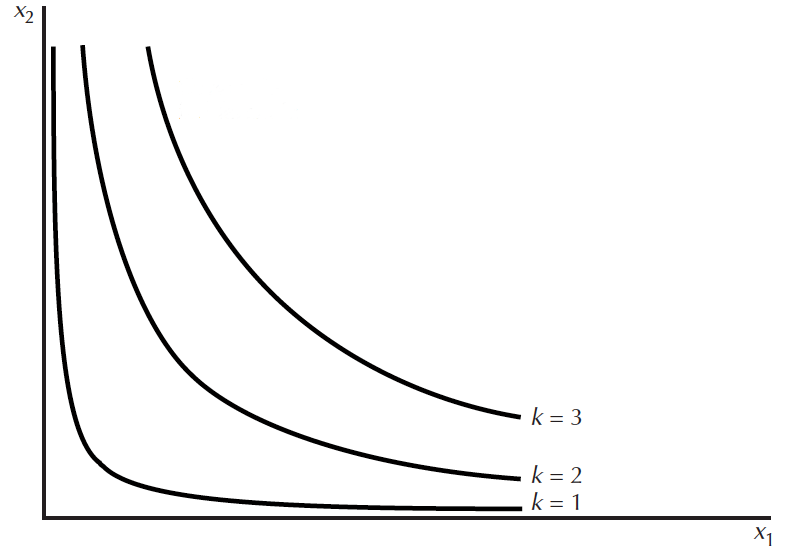
\includegraphics[width=4in]{figures2/cobbdouglas.png}
%\end{center}
%\end{frame}

\begin{frame}{Isocuantas: Tecnología Cobb-Douglas}
    \begin{figure}
\centering
\begin{subfigure}{.5\textwidth}
  \centering
  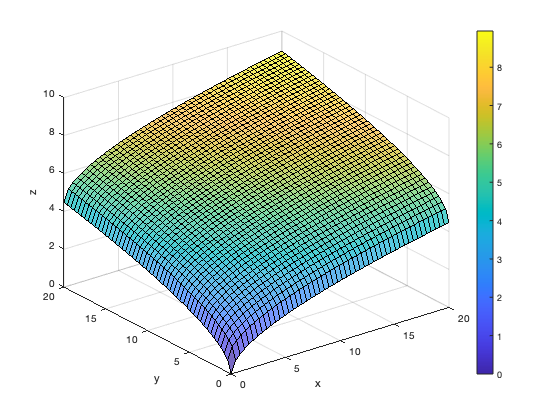
\includegraphics[width=1\linewidth]{figures2/cobbdouglas3d.png}
  \caption{Función de producción Cobb-Douglas}
  \label{fig:sub1}
\end{subfigure}%
\begin{subfigure}{.5\textwidth}
  \centering
  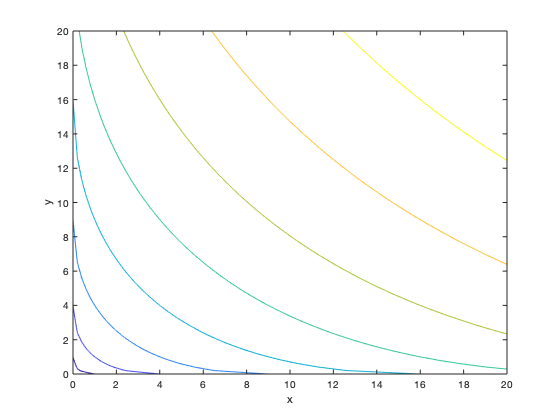
\includegraphics[width=1\linewidth]{figures2/cobbdouglaslevel.png}
  \caption{Isocuantas Cobb-Douglas si $\alpha=\beta$}
  \label{fig:sub2}
\end{subfigure}
\caption{Tecnología Cobb-Douglas si $\alpha=\beta$}
\label{fig:test}
\end{figure}
\end{frame}

\begin{frame}{Propiedades del conjunto de producción}

\begin{itemize}
    \item Vamos a estudiar dos propiedades de la tecnología (y del conjunto de producción) que son razonables de pedir: monotonicidad y convexidad (estricta o no).

\item Las tres tecnologías que vimos hasta ahora (\textbf{Leontief, sustitutos perfectos y Cobb-Douglas}) cumplen que son \textbf{monótonas y convexas}. Es decir, son tecnologías ``razonables''.

\begin{itemize}
    \item La tecnología Leontief es mónotona (pero no estrictamente) y convexa (pero no estrictamente).
    \item La tecnología de sustitutos perfectos es mónotona (estrictamente) y convexa (pero no estrictamente).
    \item Si ambos insumos $x_1>0$ y $x_2>0$, entonces la tecnología Cobb-Douglas es mónotona (estrictamente) y convexa (estrictamente).
    \item Si alguno de los insumos $x_1=0$ o $x_2=0$, entonces la tecnología Cobb-Douglas es mónotona (pero no estrictamente) y convexa (pero no estrictamente).
\end{itemize}

  \end{itemize}  
\end{frame}

\begin{frame}{Propiedades: Monotonicidad y monotonicidad estricta}
		\begin{itemize}
		\begin{block}{Monotonicidad}
  Una tecnología es monótona si partiendo de un plan de producción $(\textbf{x},y)$ se aumenta la cantidad de insumos a \textbf{x'} es entonces \textbf{factible} producir cualquier cantidad $[0,y]$ como mínimo.
  \end{block}
%		El conjunto de producci\'{o}n $Y$ satisface la  \textbf{propiedad de monotonicidad} si para cualquier plan de producci\'{o}n  $(x_{1},...,x_{n},y) \ \in Y$, el plan de producci\'{o}n $(x_1',...,x_n',y' )$ tal que $\forall i,x_i'\geq $ $ x_{i} $ y adem\'{a}s $y' \leq y$, tambi\'{e}n pertenece a $Y$.
				\begin{block}{Monotonicidad estricta}
  Una tecnología es monótona estricta si partiendo de un plan de producción factible $(\textbf{x},y)$ se aumenta la cantidad de alguno de los insumos a \textbf{x'} es entonces \textbf{factible} producir cualquier cantidad $[0,f(x')]$ donde $f(x')>y$.
  \end{block}
%\item Notar que lo que es requerido para que el conjunto de producci\'{o}n sea mon\'otono es que aumentar los insumos no haga decrecer la cantidad de producto final que se puede producir. Por lo tanto, en el caso de funciones de producci\'{o}n con un \'{u}nico insumo, basta que la misma no sea nunca decreciente.
%\item De la misma manera, en el caso de dos insumos, nunca debe ser decreciente en ninguno de ellos. 
\item ¿C\'{o}mo debe ser la frontera del conjunto de producción? \textbf{Creciente}.
\item ¿C\'{o}mo deben ser las isocuantas de conjuntos de producci\'{o}n que exhiban monotonicidad? \textbf{Decrecientes, horizontales o verticales}, es decir tienen que tener pendiente negativa, cero o no existe.
			%\item Esta propiedad se denomina a veces \textbf{eliminación gratuita}, ya que si la firma pudiera deshacerse de cualquier cantidad de un factor sin incurrir en costo alguno, no puede perjudicarle tener más del mismo.
		\end{itemize}
		\end{frame}
		

%\begin{frame}{Propiedades del conjunto de Producción}
%\begin{center}
%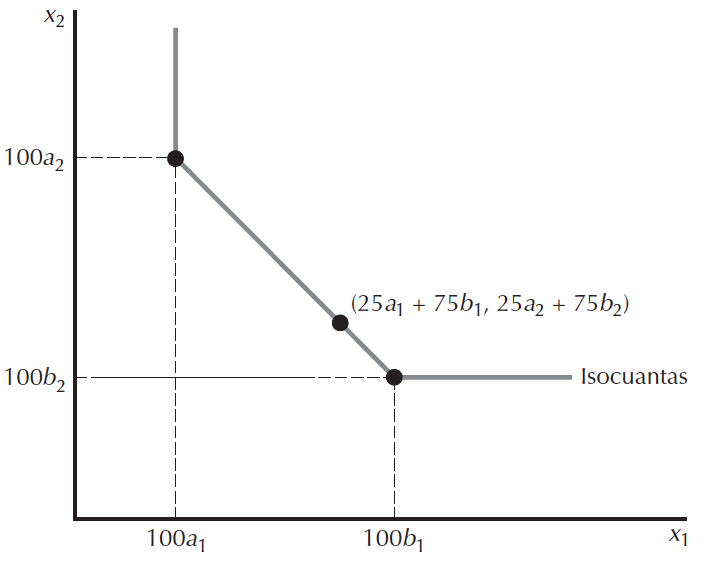
\includegraphics[width=3.7in]{figures2/isoquant.png}
%\end{center}
%\end{frame}	

\begin{frame}{Propiedades: Convexidad y convexidad estricta}
		 	\begin{block}{Convexidad}
		 	Consideremos dos planes de producción factibles $(\textbf{x},y)\in Y$ y $(\textbf{x}',y')\in Y$. La tecnología es convexa si los planes de producción ``promedio'' $(\textbf{x}'',y'')=\alpha(\textbf{x},y)+(1-\alpha)(\textbf{x}',y')$ son factibles, para cualquier valor de $\alpha\in [0,1]$.
		\end{block}
		\begin{itemize}
		\item Si la tecnolog\'{\i}a de producci\'{o}n tiene un solo factor, ¿c\'omo debe ser la frontera de producci\'{o}n? C\'{o}ncava (no necesariamente estrictamente cóncava).
		\item Si la tecnolog\'{\i}a de producci\'{o}n tiene dos factores, ¿c\'{o}mo ser\'{\i}an sus isocuantas? Convexas, aunque no hace falta que sean estrictamente convexas, pueden tener tramos horizontales o verticales.
		\end{itemize}
  \begin{block}{Convexidad estricta}
  Si la tecnología es estrictamente convexa, las isocuantas son estrictamente convexas.
  \end{block}
\end{frame}		
	

\begin{frame}{Productividad Marginal}
Supongamos que un bien se produce con la función de producción $f\left(x_{1}, x_{2}\right)$.
\medskip

A partir de un nivel de insumos $\left(x_{1}, x_{2}\right)$ consideremos aumentar la cantidad de insumo $1, x_{1}$, a $x_{1}^{\prime}$ de manera que $\triangle x_{1}=x_{1}^{\prime}-x_{1}$ \underline{manteniendo fija} la cantidad de insumo $2, x_{2}$. 
\medskip

¿Cuánto aumentará el nivel de producto final en el margen?
\begin{itemize}
    \item \textbf{Paso 1:} Al aumentar el insumo 1 en un valor de $\triangle x_{1}$ obtenemos una producción de $f\left(x_{1}+\triangle x_{1}, x_{2}\right)$. La variación en la producción es entonces $\triangle y=f\left(x_{1}+\triangle x_{1}, x_{2}\right)-f\left(x_{1}, x_{2}\right)$.
\item \textbf{Paso 2:} Dividiendo por la cantidad de insumo agregada, $\triangle x_{1}$, vemos cuánto cambia la cantidad producida por unidad:
\end{itemize}
$$
\frac{f\left(x_{1}+\Delta x_{1}, x_{2}\right)-f\left(x_{1}, x_{2}\right)}{\Delta x_{1}}
$$
\end{frame}		

\begin{frame}{Productividad Marginal}
\begin{itemize}
\item \textbf{Paso 3:} Finalmente, para ver el cambio en el margen de la cantidad producida, consideramos $\triangle x_{1} \rightarrow 0$ :
$$
\lim _{\Delta x_{1} \rightarrow 0} \frac{f\left(x_{1}+\Delta x_{1}, x_{2}\right)-f\left(x_{1}, x_{2}\right)}{\triangle x_{1}}=\frac{\partial f\left(x_{1}, x_{2}\right)}{\partial x_{1}}=P M g_{1}(x_1,x_2)
$$
\item La \textbf{Productividad Marginal del insumo} $1$ es la cantidad de producto final adicional que podemos producir al aumentar la cantidad de insumo $1$ marginalmente manteniendo las cantidades de otros insumos constante.
\item Notar que si bien la productividad marginal considera cambios $\triangle x_{1}$ ``pequeños'' a veces decimos que $PMg_{1}(x_1,x_2)$ es a\textbf{proximadamente} la cantidad adicional de producto obtenido al aumentar una unidad del insumo 1.
\end{itemize}
\end{frame}		

\begin{frame}{Productividad Marginal}
\begin{itemize}
\item Supongamos que tenemos una \textbf{tecnolog\'{\i}a que cumple monotonicidad estricta}, o sea, $PMg_i(x_1,x_2)>0$ para cualquier insumo $i$. Si aumentamos la cantidad de insumo aumentará la cantidad de bien final producida. Ahora bien, a medida que aumenta $x_1$ ¿cómo cambia $PMg_1(x_1,x_2)$? Si cada unidad adicional de $x_1$ produce cada vez %Por simplicidad, supongamos que mantenemos todos los insumos fijos menos uno, y lo aumentamos esperaremos que la cantidad de producto final que podemos producir aumente. Ahora bien, esperaremos que lo haga a tasa creciente o decreciente? Es decir, a medida que aumentamos el insumo, la cantidad de bien final que produce por unidad extra, es mayor o menor?
\small
\item menos unidades de $y$, entonces $(\frac{\partial PMg_{1}(x_1,x_2)}{\partial x_{1}}<0)$ diremos que la productividad marginal del factor es decreciente o que tenemos rendimientos marginales decrecientes. 
\item más unidades de $y$, entonces  $(\frac{\partial PMg_{1}(x_1,x_2)}{\partial x_{1}}>0)$ diremos que la productividad marginal del factor es creciente o que tenemos rendimientos marginales crecientes.
\item las mismas unidades de $y$, entonces  $(\frac{\partial PMg_{1}(x_1,x_2)}{\partial x_{1}}=0)$ diremos que la productividad marginal del factor es constante o que tenemos rendimientos marginales constantes.
\item Normalmente cabe esperar que el producto marginal de un factor disminuya a medida que se emplee una cantidad cada vez mayor de él. Esto se conoce como \textbf{ley de rendimientos marginales decrecientes}.
%\item Normalmente cabe esperar que el producto marginal de un factor disminuya a medida que se emplee una cantidad cada vez mayor de él. Este fenómeno se denomina \textbf{ley del producto marginal decreciente}. En realidad, no es una ``ley$"$, sino meramente un rasgo común a casi todos los procesos de producción. Es importante subrayar que la ley del producto marginal decreciente sólo se cumple cuando todos los demás factores se mantienen fijos.

\end{itemize}
\end{frame}	

\begin{frame}{Tasa Marginal de Sustitución Técnica}
	\begin{itemize}
\item ¿Qué es $TMST(x_1,x_2)$? Es la cantidad de unidades del insumo $2$ adicionales tiene que comprar la firma si, con el objetivo de mantener la cantidad $\overline{y}$ fija sobre una isocuanta, si deja de utilizar una unidad del insumo $1$ (medido en unidades de insumo $2$). 

\item Entonces $TMST(x_1,x_2)$ mide el costo de oportunidad sobre una isocuanta de nivel $\overline{y}$ de utilizar una unidad del insumo $1$.
%	\item Sobre una isocuanta se encuentran las combinaciones de factores que, a través de la tecnología, producen la misma cantidad de producto.
\item \textbf{Sobre una isocuanta} las firmas enfrentan el \textbf{costo de oportunidad de elegir utilizar un insumo, decidiendo en el margen usar menos del otro manteniendo constante la cantidad producida}. Llamamos a este costo de oportunidad \textbf{tasa marginal de sustitución técnica}.
%\item Si una firma produce una cantidad $\overline{y}$ (sobre una isocuanta) icuál es el criterio para elegir una combinación de insumos $(x_{1}, x_{2})$ sobre la isocuanta?
\item ¿Por qué este costo de oportunidad se llama TMST$(x_1,x_2)$?
	\end{itemize}	
\end{frame}		

 \begin{frame}{Tasa Marginal de Sustitución Técnica}
 Gráficamente, pasamos de una combinación de insumos \color{rosee} A \color{black} a una combinación de insumos \color{rosee} B\color{black}. ¿cuánto vale aproximadamente la TMST$(x_1,x_2)$?\footnote{Note que aquí llamé $q$ en vez de $\overline{y}$ a la cantidad producida en la isocuanta.}
 
 \begin{center}
     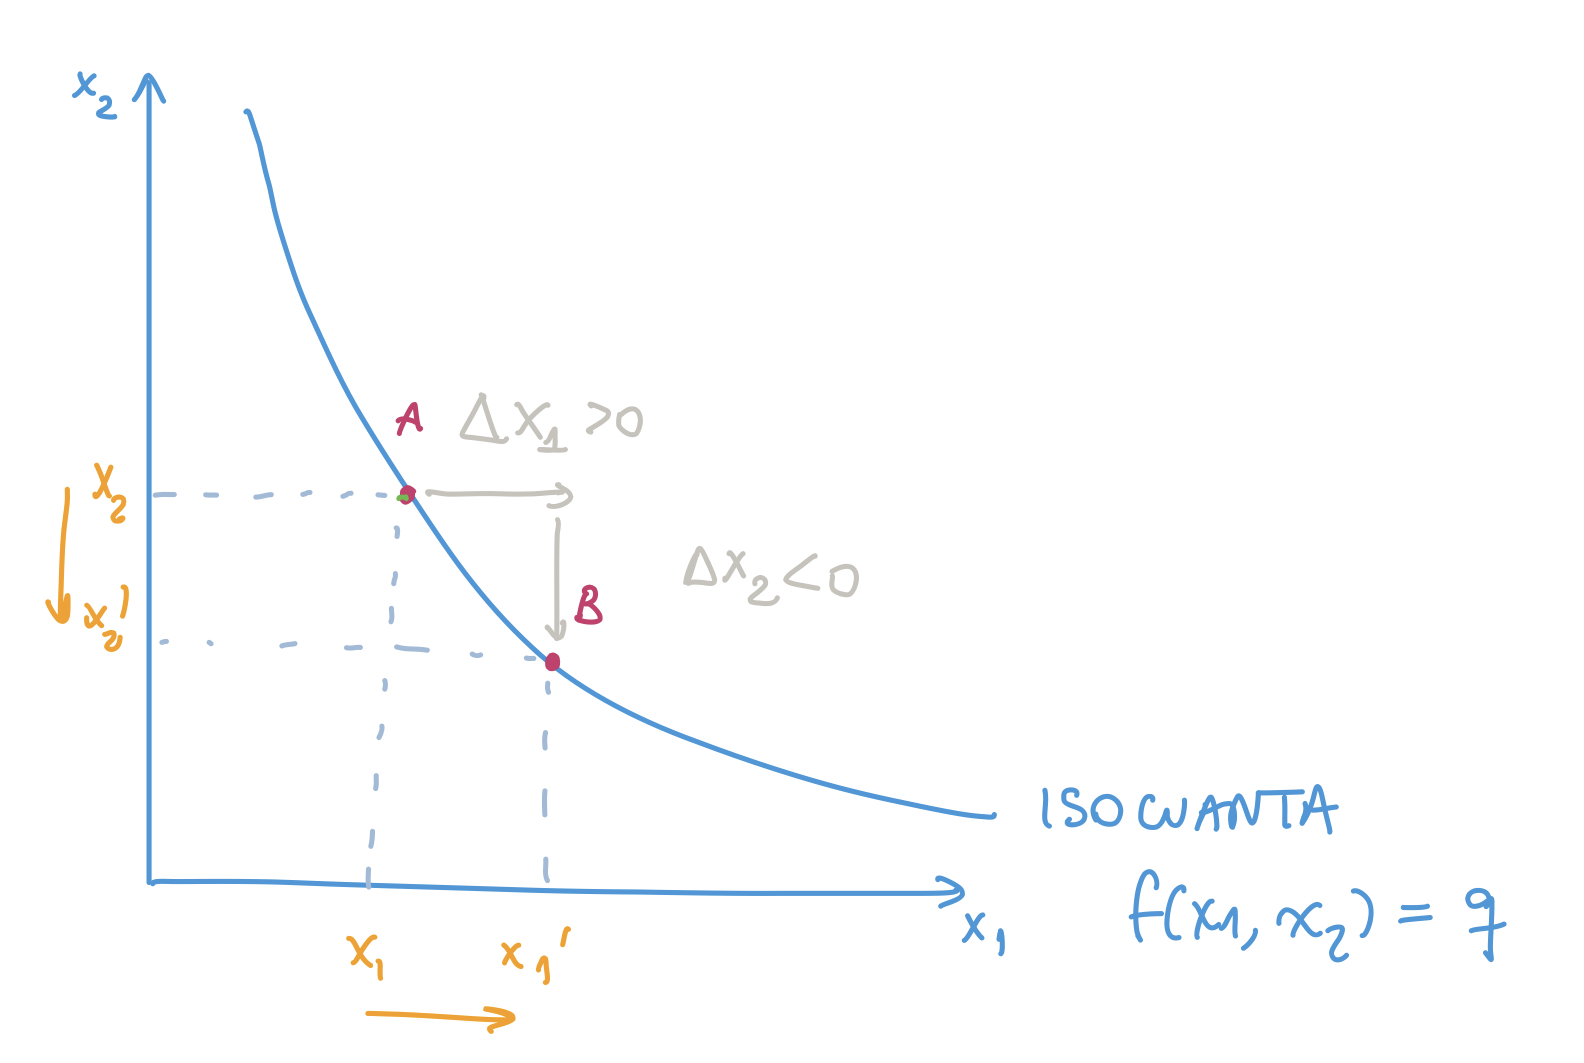
\includegraphics[scale=0.15]{figures2/TMST.jpeg}
 \end{center}
 \end{frame}

\begin{frame}{Tasa Marginal de Sustitución Técnica}
	\begin{itemize}
			\item Para obtener la TMST,  diferenciamos totalmente la funci\'on de producci\'on:
		$$\triangle y\equiv\triangle f(x_{1},x_{2})=PMg_{1}(x_1,x_2)\triangle x_{1}+PMg_{2}(x_1,x_2)\triangle x_{2}$$
		\item Recordando que sobre una isocuanta $\triangle y=0$, entonces:
		$$0=\triangle f(x_{1},x_{2})=PMg_{1}(x_1,x_2)\triangle x_{1}+PMg_{2}(x_1,x_2)\triangle x_{2}$$
		$$\Longrightarrow \frac{\triangle x_{2}}{\triangle x_{1}}=-\frac{PMg_{1}(x_1,x_2)}{PMg_{2}(x_1,x_2)}$$
		\item Si consideramos cambios de insumo 1 cada vez menores, que tiendan a cero:
		$$\lim_{\triangle_1 \rightarrow 0} \frac{\triangle x_{2}}{\triangle x_{1}}=\frac{\partial x_{2}}{\partial x_{1}}=-\frac{PMg_{1}(x_1,x_2)}{PMg_{2}(x_1,x_2)}=TMST(x_1,x_2)$$
	\end{itemize}	
\end{frame}			

\begin{frame}{Tasa Marginal de Sustitución Técnica}
¿En qué unidades y qué información nos da la TMST$(x_1,x_2)$?

\begin{itemize}
    \item \color{red} La TMST$(x_1,x_2)$ mide \textbf{la cantidad de unidades del insumo 2} que hay que ceder para aumentar la cantidad de insumo 1 en una unidad y así mantener la producción en el mismo nivel $y$.
    \item \color{blue} La TMST$(x_1,x_2)$ mide \textbf{la cantidad de unidades del insumo 2} que se puede aumentar para cuando se deja de usar una unidad del insumo 1 y así mantener la producción en el mismo nivel $y$.
    \item \color{black}Es decir, la TMST$(x_1,x_2)$ mide el costo de oportunidad de usar una unidad \color{red} más \color{blue}(menos) \color{black} del insumo 1.
    \item Normalmente diremos que la TMST$(x_1,x_2)$ será decreciente a medida que aumenta $x_1$. ¿Por qué ocurre esto? Porque cuando se tiene una cantidad muy alta de $x_1$ hay que ceder pocas unidades del insumo 2 con tal de aumentar la cantidad de insumo 1 para que la producción quede constante.
\end{itemize}

\end{frame}
%\begin{frame}{Tasa Marginal de Sustitución Técnica}
%	\begin{itemize}
%		\item La tasa marginal de sustituci\'{o}n t\'{e}cnica $(TMST)$ ser\'{a} decreciente si la cantidad de insumo 2 con la que tenemos que compensar una ca\'ida del insumo 1 de forma tal de mantener el producto constante es cada vez mayor a medida que cae la cantidad de insumo 1. 
%\item Por lo tanto, la forma de la isocuanta que representa tecnolog\'{\i}as con esta caracter\'{\i}stica debe ser decreciente a tasa decreciente a medida que aumentamos el insumo 1, es decir, convexa.
%\item Los supuestos de la $TMST$ decreciente y del producto marginal decreciente están estrechamente relacionados entre sí, pero no son exactamente lo mismo. El producto marginal decreciente es un supuesto sobre la forma en que varía el producto marginal cuando aumenta la cantidad empleada de un factor y se mantiene fija la del otro. La $TMST$ se refiere a la forma en que varía el cociente de los productos marginales, es decir, la pendiente de la isocuanta.
%	\end{itemize}
%\end{frame}	

\begin{frame}{Rendimientos a Escala}
	\begin{itemize}
		\item Supongamos ahora que aumentamos el valor de todos los insumos en la misma proporción $(tx_1,tx_2)$. Si la tecnología de producción es monótona, entonces sabemos que la producción aumentará. La pregunta es cuánto y cómo se compara con aumentar la producción multiplicando por la misma escala $tf(x_1,x_2)$.
  
  \begin{itemize}
      \item \small{El conjunto de producci\'on $Y$ exhibe \textbf{rendimientos crecientes a escala} (IRS) si: }
		\[\forall t > 1, \ f(t\textbf{x})>tf(\textbf{x})\]
  \item \small{El conjunto de producci\'on $Y$ exhibe \textbf{rendimientos constantes a escala} (CRS) si: }
		\[\forall t > 1, \ f(t\textbf{x})=tf(\textbf{x})\]
  \small{El conjunto de producci\'on $Y$ exhibe r\textbf{endimientos decrecientes a escala} (DRS) si: }
		\[\forall t > 1, \ f(t\textbf{x})<tf(\textbf{x})\]
  \end{itemize}
\end{itemize}	
\end{frame}

\begin{frame}{Rendimientos a Escala}
\begin{thm}
	Si la función de producci\'on $f$ es estrictamente c\'oncava, entonces el conjunto de producción $Y$ es convexo. Si además $f(0)=0$, entonces $Y$ tiene rendimientos decrecientes a escala.
\end{thm}
\begin{thm}
	Si la función de producci\'on $f$ es estrictamente convexa, entonces el conjunto de producción $Y$ no es convexo. Si además $f(0)=0$, entonces $Y$ tiene rendimientos crecientes a escala.
\end{thm}
\begin{thm}
	Si la función de producci\'on $f$ es lineal, entonces el conjunto de producción $Y$ es convexo. Si además $f(0)=0$, entonces $Y$ tiene rendimientos constantes a escala.
\end{thm}
\end{frame}

\begin{frame}{Retornos a Escala: Ejemplos}
\textbf{Tecnolog\'ia Leontief}: $f(x_{1},x_{2})=[min\lbrace a_{1}x_{1},a_{2}x_{2}\rbrace]^{\alpha}$, $a_{i}>0,\alpha>0$. Los rendimientos a escala de esta funci\'on dependen del valor de $\alpha$:
\begin{itemize}
	\item $\alpha < 1 \implies$ $f(x_1,x_2)$ tiene rendimientos decrecientes a escala.
	\item $\alpha = 1 \implies$ $f(x_1,x_2)$ tiene rendimientos constantes a escala.
	\item $\alpha > 1 \implies$ $f(x_1,x_2)$ tiene rendimientos crecientes a escala.
\end{itemize}

\textbf{Tecnolog\'ia Cobb-Douglas}: $f(x_{1},x_{2})=x_{1}^{\alpha}x_{2}^{\beta}$, $\alpha,\beta>0$. Los rendimientos a escala dependen del valor de $\alpha+\beta$.
\begin{itemize}
	\item $\alpha+\beta < 1 \implies$ $f(x_1,x_2)$ tiene rendimientos decrecientes a escala.
	\item $\alpha+\beta  = 1 \implies$ $f(x_1,x_2)$ tiene rendimientos constantes a escala.
	\item $\alpha +\beta > 1 \implies$ $f(x_1,x_2)$ tiene rendimientos crecientes a escala.
\end{itemize}
\end{frame}

\begin{frame}{Tecnologías Homogéneas y Homotéticas}\small
\begin{itemize}[leftmargin=*]
	    \item \textbf{Definición:} Una función es \textbf{homogénea de grado k} $(HOD \,k)$ si $f(t\textbf{x})=t^{k}f(\textbf{x})$. Es decir, que al aumentar la escala de los insumos multiplicando por $t$ multiplica la escala de la cantidad producida por $t^k$. Entonces vale que $TMST(x)=TMST(tx)$ y que la isocuanta de nivel $t^ky$ se puede alcanzar mutiplicando todos los insumos de la isocuanta de nivel $y$ por $t$.
\item \textbf{Propiedad:} Una función exhibe rendimientos constantes a escala si y sólo si es homogénea de grado 1. Entonces vale que $f(tx)=tf(x)$ y que $TMST(x)=TMST(tx)$ y que la isocuanta de nivel $ty$ se puede alcanzar mutiplicando todos los insumos de la isocuanta de nivel $y$ por $t$.
\item \textbf{Definición:} Una función $g:\mathbb{R}\rightarrow\mathbb{R}$ es una \textbf{transformación monótona} si $g$ es una función estrictamente creciente.
\item \textbf{Definición:} Una función $f(\textbf{x})$ es una función \textbf{homotética} si $f(\textbf{x})=g(h(\textbf{x}))$, donde $h(\cdot)$ es homogénea de grado $k$ y $g(\cdot)$ es estrictamente creciente. Es decir, si $f$ es una transformación monótona de una función $HOD \,k$. Entonces vale que $TMST(x)=TMST(tx)$ y que la isocuanta de nivel $ty$ se puede alcanzar mutiplicando todos los insumos de la isocuanta de nivel $y$ por algún múltiplo (no se puede saber de antemano cuánto vale).	
\end{itemize}
\end{frame}

\begin{frame}{Tecnologías Homogéneas y Homotéticas}
\begin{center}
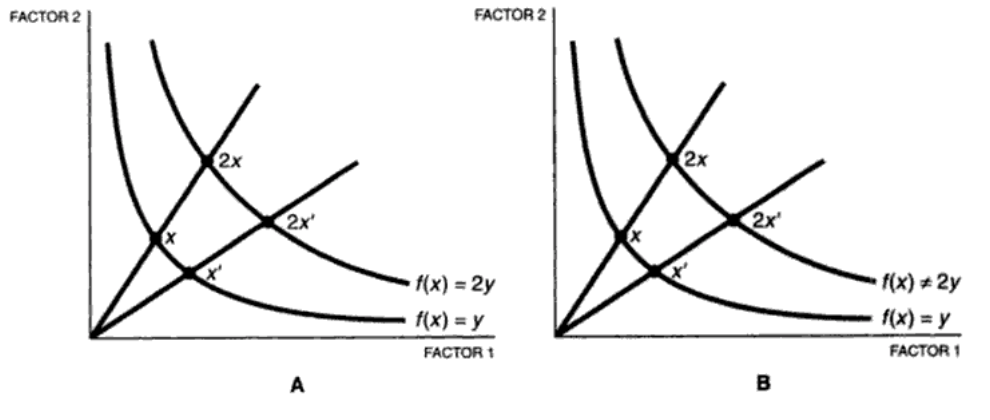
\includegraphics[width=4.5in]{figures2/homoteticas.png}
\end{center}\small
\textbf{Importante:} Para las tecnologías homogéneas y homotéticas, la $TMST(x_1,x_2)$ es independiente de la escala de producción, es decir, solamente dependen de $\frac{x_1}{x_2}$. Las funciones a) homog\'{e}neas HOD1 (figura $A$) y b) homot\'{e}ticas u c) HOD $k$ ($k \neq 1$) (figura $B$) difieren en que, al aumentar la escala de producción $(tx_1, tx_2)$ producen: a) $tf(x_1,x_2)$, b) $y$ mayor que antes -no podemos especificar- c) a) $t^kf(x_1,x_2)$.
\end{frame}

%\begin{frame}{Tecnologías Homogéneas y Homotéticas}
%\small
%\begin{itemize}
%\item En el caso de la \textbf{funci\'{o}n homog\'{e}nea}, las isocuantas no son sino ampliaciones de una \'{u}nica isocuanta. En particular, si $f(\textbf{x})$ es homog\'{e}nea de grado 1, entonces si $\textbf{x}$ y $\textbf{x}' $ pueden generar $y$
%unidades de producci\'{o}n, $t\textbf{x}$ y $t\textbf{x}' $ pueden generar $ty$ unidades.
%\item Una \textbf{funci\'{o}n homot\'{e}tica} u homogénea HOD $k$ ($k\neq 1$) posee una propiedad muy parecida: si $\textbf{x}$ y $\textbf{x}' $ generan el mismo nivel de producci\'{o}n, $t\textbf{x}$ y $t\textbf{x}'$ puede generar el mismo nivel de producci\'{o}n, pero no necesariamente un nivel de producci\'{o}n $t$ veces superior al inicial. %Las isocuantas de una tecnolog\'{\i}a homot\'{e}tica son exactamente iguales que las de una tecnolog\'{\i}a homog\'{e}na; s\'olo son diferentes los niveles de producci\'{o}n correspondientes.
%\item La propiedad relevante para estas tecnologías es que en el punto donde se minimizan costos, la pendiente de la isocuanta tiene que ser igual a la pendiente de la recta de isocosto en valor absoluto $\frac{w_1}{w_2}$. Entonces si $(x_1, x_2)$ minimizan costos sobre la isocuanta $\bar{y}$ cuando los costos son $w_1$ y $w_2$, si se quisiera producir $t\bar{y}$ entonces $(kx_1, kx_2)$ minimizan costos. Notar que $t=k$ solamente si %$f(x_1,x_2)$ es HOD 1, notar que $k=t
%^\ell$ si $f(x_1,x_2)$ es HOD $\ell$ y si $f(x_1,x_2)$ es homotética, no sabemos qué relación hay entre $k$ y $t$.
%\end{itemize}
%\end{frame}

{
\setbeamercolor{background canvas}{bg=}
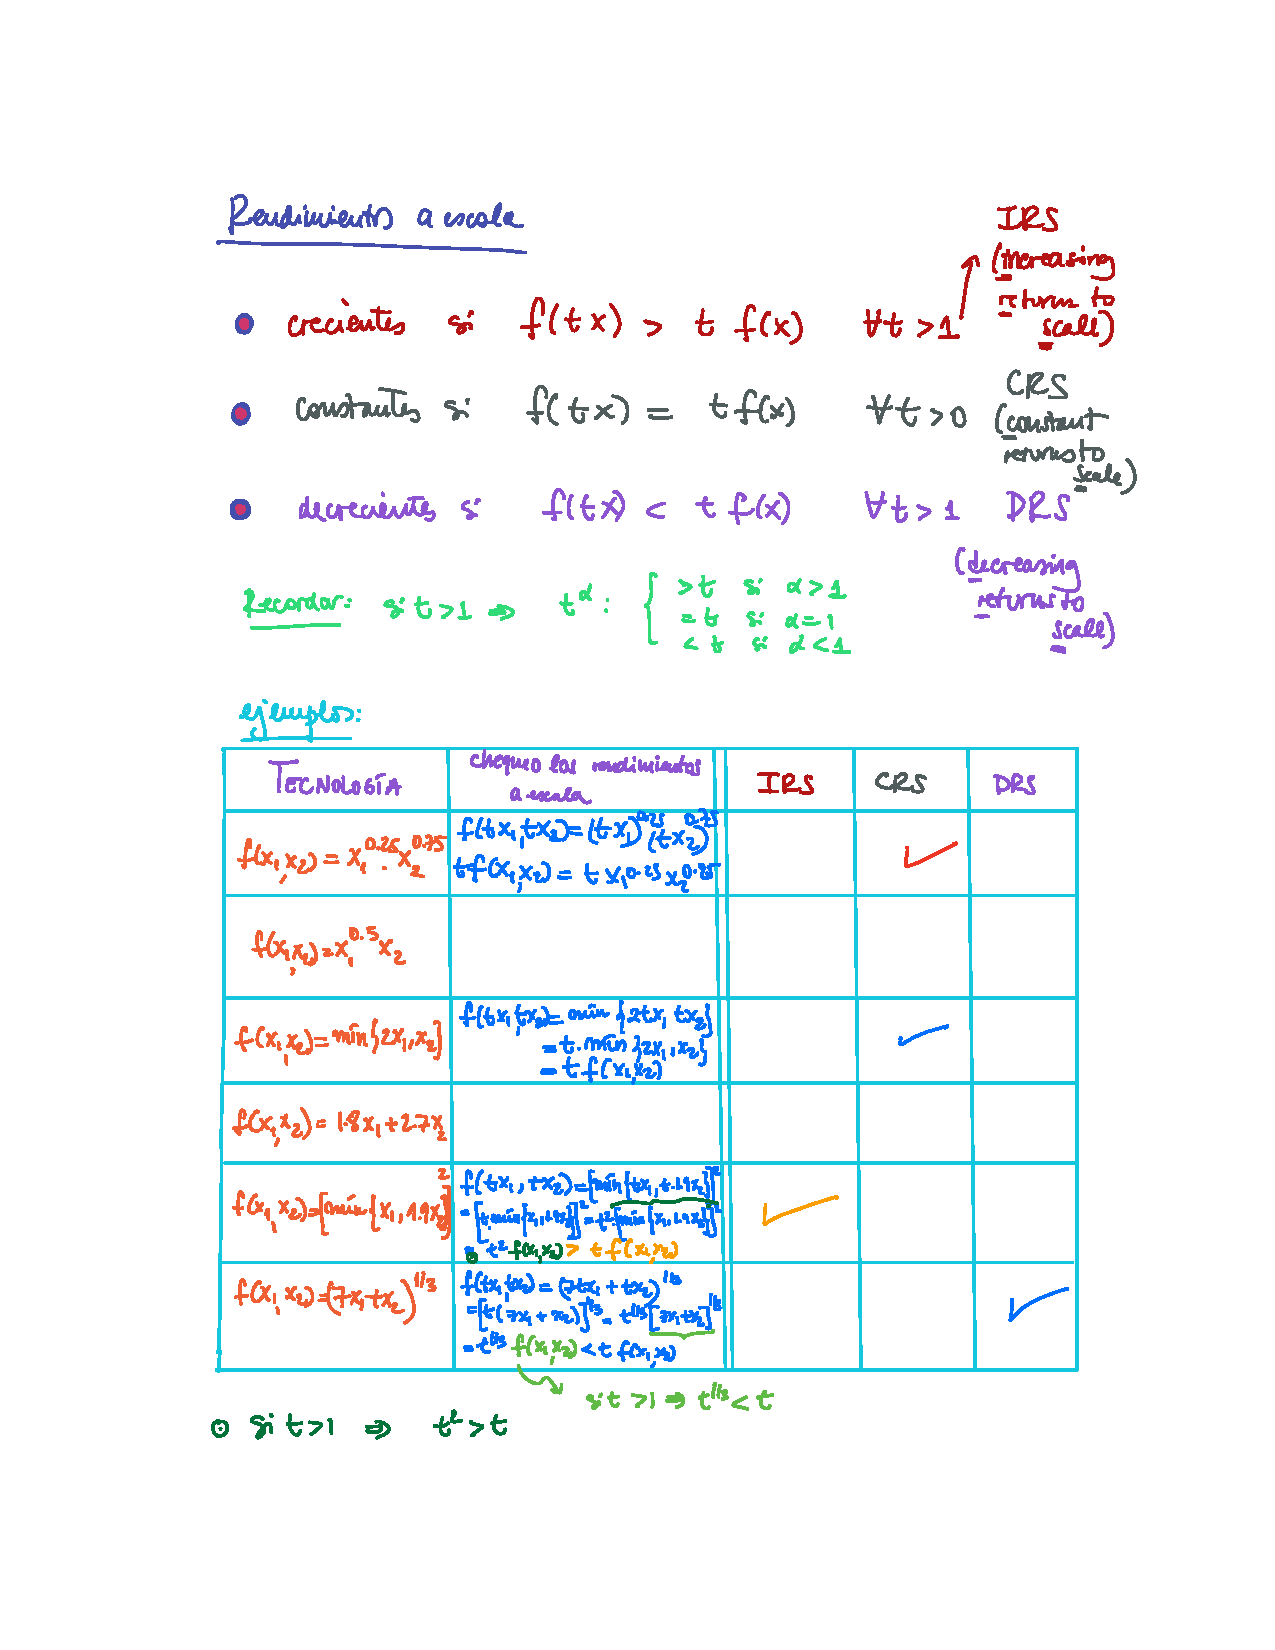
\includepdf[pages=-,fitpaper]{figures2/extra.pdf}
}
\end{document}















\begin{frame}{Ap\'endice: Elasticidad de Sustituci\'on}
\begin{itemize}
\item La $TMST$ mide la pendiente de una isocuanta. La elasticidad de sustitución mide su curvatura. Más concretamente, la elasticidad de sustituci\'on mide la variación porcentual del cociente entre los factores dividida por la variaci\'on porcentual de la $TMST$, manteniéndose fijo el nivel de producción.
\item Si suponemos que $\triangle (x_2/ x_1)$ es la variación del cociente entre los factores y $\triangle TMST$ es la variación de la $TMST$, podemos expresar ésta de la manera siguiente:
\begin{center}
$\sigma=\dfrac{\frac{\triangle (x_2/ x_1)}{x_2/x_1}}{\frac{\triangle (TMST)}{TMST}}$
\end{center}
\end{itemize}
\end{frame}

\begin{frame}{Ap\'endice: Elasticidad de Sustituci\'on}
\begin{itemize}
\item La elasticidad de sustitución es una medida relativamente natural de la curvatura: se pregunta cómo varía el cociente entre las cantidades de factores cuando varía la pendiente de la isocuanta. Si una pequeña variación de la pendiente provoca una gran variación del cociente entre las cantidades de factores, la isocuanta es relativamente horizontal, lo que significa
que la elasticidad de sustitución es grande.
\item En la práctica, suponemos que la variación porcentual es muy pequeña y tomamos
el límite de esta expresión cuando $\triangle$ tiende a cero. Por lo tanto, la expresión de $\sigma$ a se convierte en:
\begin{center}
$\sigma=\dfrac{\frac{d (x_2/ x_1)}{x_2/x_1}}{\frac{d (TMST)}{TMST}}$
\end{center}
\end{itemize}
\end{frame}

\begin{frame}{Ap\'endice: Elasticidad de Sustituci\'on}
\begin{itemize}
\item A menudo resulta útil calcular $\sigma$ utilizando la derivada logarítmica. En general,
si $y = g(x)$, la elasticidad de $y$ con respecto a $x$ se refiere a la variación de $y$ provocada
por una (pequeña) variación porcentual de $x$. Es decir,
\begin{center}
$\epsilon=\dfrac{\frac{dy}{y}}{\frac{dx}{x}}=\frac{dy}{dx}\frac{x}{y}$
\end{center}
\item Siempre que $x$ e $y$ sean positivos, esta derivada puede expresarse de la forma siguiente:
\begin{center}
$\epsilon=\frac{d\ln(y)}{d\ln(x)}$
\end{center}
\item Aplicando este resultado a la elasticidad de sustitución, obtenemos la siguiente
expresión:
\begin{center}
$\sigma=\dfrac{d\ln(x_2/x_1)}{d\ln|TMST|}$
\end{center}
\end{itemize}
\end{frame}

\begin{frame}{Ap\'endice: Elasticidad de Sustituci\'on}
\begin{itemize}
\item Tomemos el ejemplo de la funci\'on $f(x_1,x_2)=x_1^{\alpha}x_2^{1-\alpha}$. Tenemos que $TMST=-\frac{\alpha}{1-\alpha}\frac{x_2}{x_1}$. Luego,
\begin{center}
$\frac{x_2}{x_1}=-\frac{1-\alpha}{\alpha}TMST$
\end{center}
Tomando logaritmo ambos miembros:
\begin{center}
$\ln\left(\frac{x_2}{x_1}\right)=\ln\left(\frac{1-\alpha}{\alpha}\right)+\ln|TMST|$
\end{center}
Por lo tanto,
\begin{center}
$\sigma=\dfrac{d\ln(x_2/x_1)}{d\ln|TMST|}=1$
\end{center}
\end{itemize}
\end{frame}

\begin{frame}{Ap\'endice: Tecnolog\'ia CES}
	\begin{itemize}
		\item Tecnolog\'ia de producci\'on un poco m\'as general y es de la forma:
		$$f(x_{1},x_{2})=(x_{1}^{\rho}+x_{2}^{\rho})^{\frac{1}{\rho}}$$
		Tenemos que $TMST=-\left(\frac{x_1}{x_2}\right)^{\rho -1} \Leftrightarrow \frac{x_2}{x_1}=|TMST|^{\frac{1}{1-\rho}}$\\
		Luego,
		\begin{center}
		$\ln\left(\frac{x_2}{x_1}\right)=\frac{1}{1-\rho}\ln|TMST|$
		\end{center}
		Por lo tanto,
\begin{center}
$\sigma=\dfrac{d\ln(x_2/x_1)}{d\ln|TMST|}=\frac{1}{1-\rho}$
\end{center}
\item Si $\rho=1$, la funci\'on de producci\'on se transforma en una l\'ineal (sustitutos).
		\item Si $\rho\rightarrow 0$, las isocuantas se asemejan a una Cobb-Douglas.
		\item Si $\rho\rightarrow -\infty$, las isocuantas se asemejan a una Leontief.
		\end{itemize}
		\end{frame}
